\documentclass[11pt,a4paper]{article}

% packages
  \usepackage{a4wide}
  \usepackage{tikz}
  \usepackage{amsmath}
  \usepackage{mathtools}

  \tikzset{st/.style = {circle, thick, minimum size=5.0mm, inner sep=0pt, draw},
           we/.style = {circle, thick, minimum size=2.0mm, inner sep=0pt, draw},
           b/.style = {circle, fill,  minimum size=1.8mm, inner sep=0pt, draw},
           a/.style = {        thick, minimum size=2.0mm, inner sep=0pt, draw}}

\pagestyle{empty}

\title{Graph Algorithms and Complexity Theory - Coursework 1}
\author{Oskar Mampe}
\date{Semester 1 Session 2019--2020}

\begin{document}

\maketitle

\thispagestyle{empty}

The following minimal cut and maximum flow can be calculated by doing the following. Residual capacities and an augmenting path indicated by bold edges.

\begin{center}
%%%%%%%%%%%%%% ORIGINAL %%%%%%%%%%%%%%
Original Network:\\
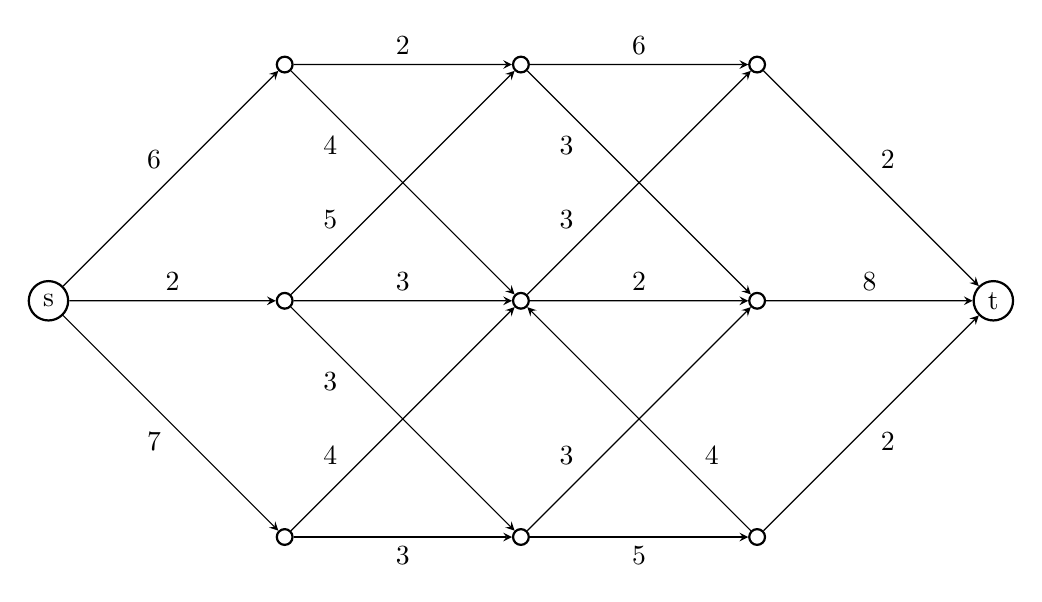
\begin{tikzpicture}[scale=1.5, >=stealth]
    \node[st] (s) at (0,2) {s};
    \node[we] (a) at (2,0) {}; \node[we] (b) at (2,2) {}; \node[we] (c) at (2,4) {}; 
    \node[we] (d) at (4,0) {}; \node[we] (e) at (4,2) {}; \node[we] (f) at (4,4) {}; 
    \node[we] (g) at (6,0) {}; \node[we] (h) at (6,2) {}; \node[we] (i) at (6,4) {}; 
    \node[st] (t) at (8,2) {t};
    \draw[->] (s) to[edge label'=7, pos=.50] (a);
    \draw[->] (s) to[edge label =2, pos=.50] (b);
    \draw[->] (s) to[edge label =6, pos=.50] (c);
    \draw[->] (a) to[edge label'=3, pos=.50] (d);
    \draw[->] (b) to[edge label =3, pos=.50] (e);
    \draw[->] (c) to[edge label =2, pos=.50] (f);
    \draw[->] (a) to[edge label =4, pos=.25] (e);
    \draw[->] (b) to[edge label =5, pos=.25] (f);
    \draw[->] (c) to[edge label'=4, pos=.25] (e);
    \draw[->] (b) to[edge label'=3, pos=.25] (d);
    \draw[->] (d) to[edge label'=5, pos=.50] (g);
    \draw[->] (e) to[edge label =2, pos=.50] (h);
    \draw[->] (f) to[edge label =6, pos=.50] (i);
    \draw[->] (d) to[edge label =3, pos=.25] (h);
    \draw[->] (e) to[edge label =3, pos=.25] (i);
    \draw[->] (f) to[edge label'=3, pos=.25] (h);
    \draw[<-] (e) to[edge label =4, pos=.75] (g);
    \draw[->] (g) to[edge label'=2, pos=.50] (t);
    \draw[->] (h) to[edge label =8, pos=.50] (t);
    \draw[->] (i) to[edge label =2, pos=.50] (t);    
  \end{tikzpicture}
  %%%%%%%%%%%%%% FIRST PASS %%%%%%%%%%%%%%
  \newpage
  \subsection*{First Pass}
  Original Network:\\
	\hfill
  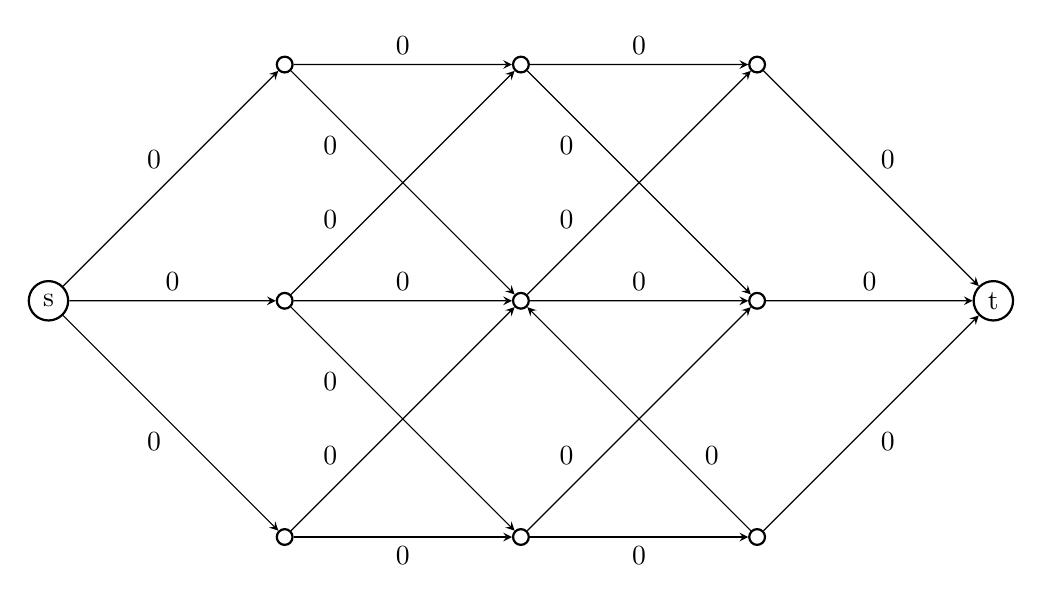
\begin{tikzpicture}[scale=1.5, >=stealth]
    \node[st] (s) at (0,2) {s};
    \node[we] (a) at (2,0) {}; \node[we] (b) at (2,2) {}; \node[we] (c) at (2,4) {}; 
    \node[we] (d) at (4,0) {}; \node[we] (e) at (4,2) {}; \node[we] (f) at (4,4) {}; 
    \node[we] (g) at (6,0) {}; \node[we] (h) at (6,2) {}; \node[we] (i) at (6,4) {}; 
    \node[st] (t) at (8,2) {t};
    \draw[->] (s) to[edge label'=0, pos=.50] (a);
    \draw[->] (s) to[edge label =0, pos=.50] (b);
    \draw[->] (s) to[edge label =0, pos=.50] (c);
    \draw[->] (a) to[edge label'=0, pos=.50] (d);
    \draw[->] (b) to[edge label =0, pos=.50] (e);
    \draw[->] (c) to[edge label =0, pos=.50] (f);
    \draw[->] (a) to[edge label =0, pos=.25] (e);
    \draw[->] (b) to[edge label =0, pos=.25] (f);
    \draw[->] (c) to[edge label'=0, pos=.25] (e);
    \draw[->] (b) to[edge label'=0, pos=.25] (d);
    \draw[->] (d) to[edge label'=0, pos=.50] (g);
    \draw[->] (e) to[edge label =0, pos=.50] (h);
    \draw[->] (f) to[edge label =0, pos=.50] (i);
    \draw[->] (d) to[edge label =0, pos=.25] (h);
    \draw[->] (e) to[edge label =0, pos=.25] (i);
    \draw[->] (f) to[edge label'=0, pos=.25] (h);
    \draw[<-] (e) to[edge label =0, pos=.75] (g);
    \draw[->] (g) to[edge label'=0, pos=.50] (t);
    \draw[->] (h) to[edge label =0, pos=.50] (t);
    \draw[->] (i) to[edge label =0, pos=.50] (t);    
  \end{tikzpicture}
  \hspace*{\fill}
  
  Residual Network:\\
    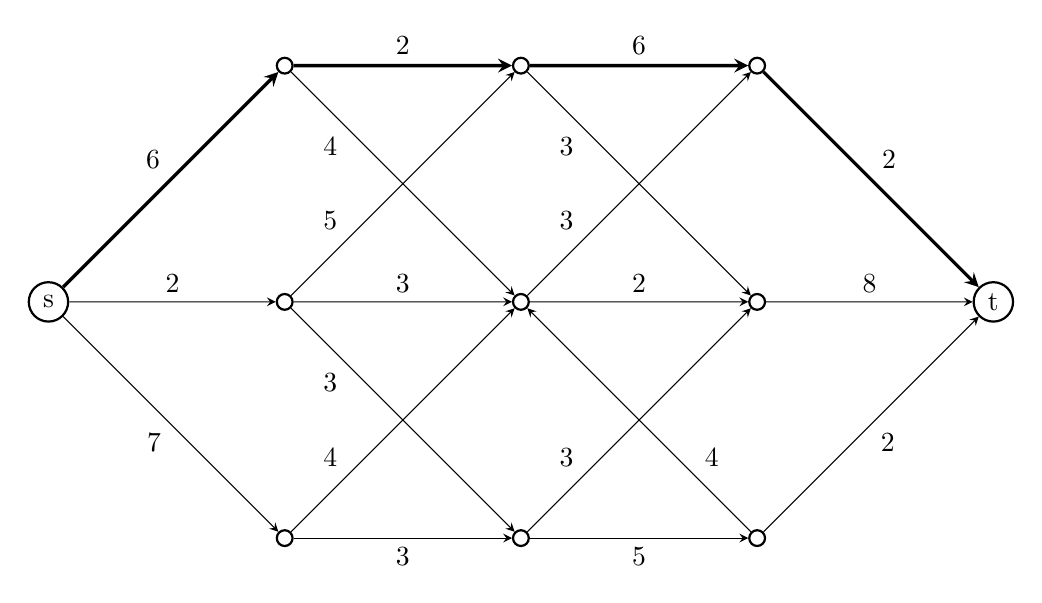
\begin{tikzpicture}[scale=1.5, >=stealth]
    \node[st] (s) at (0,2) {s};
    \node[we] (a) at (2,0) {}; \node[we] (b) at (2,2) {}; \node[we] (c) at (2,4) {}; 
    \node[we] (d) at (4,0) {}; \node[we] (e) at (4,2) {}; \node[we] (f) at (4,4) {}; 
    \node[we] (g) at (6,0) {}; \node[we] (h) at (6,2) {}; \node[we] (i) at (6,4) {}; 
    \node[st] (t) at (8,2) {t};
    \draw[->] (s) to[edge label'=7, pos=.50] (a);
    \draw[->] (s) to[edge label =2, pos=.50] (b);
    \draw[->, very thick] (s) to[edge label =6, pos=.50] (c);
    \draw[->] (a) to[edge label'=3, pos=.50] (d);
    \draw[->] (b) to[edge label =3, pos=.50] (e);
    \draw[->, very thick] (c) to[edge label =2, pos=.50] (f);
    \draw[->] (a) to[edge label =4, pos=.25] (e);
    \draw[->] (b) to[edge label =5, pos=.25] (f);
    \draw[->] (c) to[edge label'=4, pos=.25] (e);
    \draw[->] (b) to[edge label'=3, pos=.25] (d);
    \draw[->] (d) to[edge label'=5, pos=.50] (g);
    \draw[->] (e) to[edge label =2, pos=.50] (h);
    \draw[->, very thick] (f) to[edge label =6, pos=.50] (i);
    \draw[->] (d) to[edge label =3, pos=.25] (h);
    \draw[->] (e) to[edge label =3, pos=.25] (i);
    \draw[->] (f) to[edge label'=3, pos=.25] (h);
    \draw[<-] (e) to[edge label =4, pos=.75] (g);
    \draw[->] (g) to[edge label'=2, pos=.50] (t);
    \draw[->] (h) to[edge label =8, pos=.50] (t);
    \draw[->, very thick] (i) to[edge label =2, pos=.50] (t);    
  \end{tikzpicture}
  
  \newpage
  %%%%%%%%%%%%%% SECOND PASS %%%%%%%%%%%%%%
  \subsection*{Second Pass}
  Original Network:\\
  	\hfill
    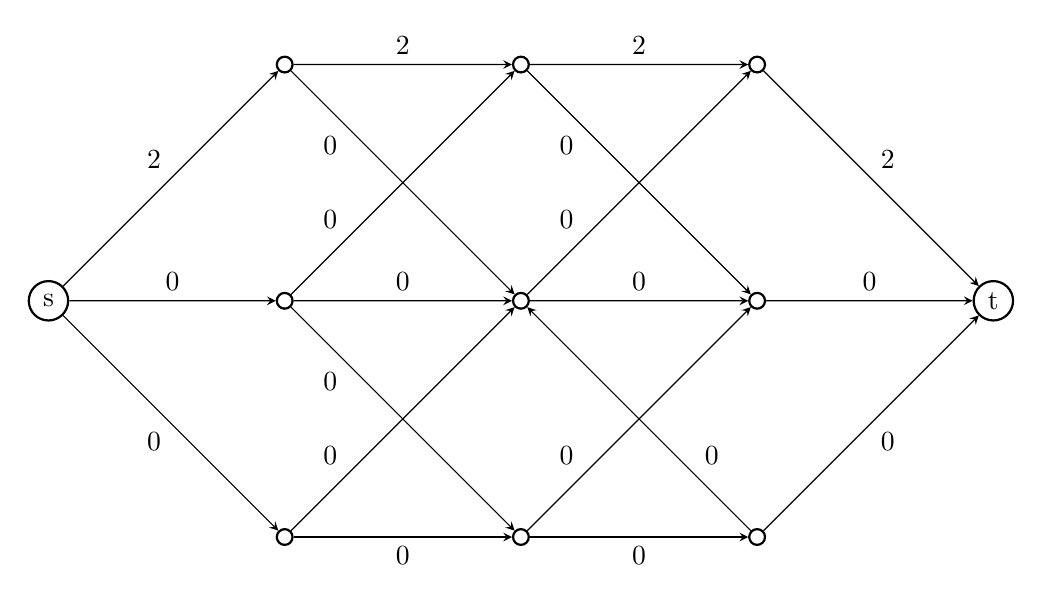
\begin{tikzpicture}[scale=1.5, >=stealth]
    \node[st] (s) at (0,2) {s};
    \node[we] (a) at (2,0) {}; \node[we] (b) at (2,2) {}; \node[we] (c) at (2,4) {}; 
    \node[we] (d) at (4,0) {}; \node[we] (e) at (4,2) {}; \node[we] (f) at (4,4) {}; 
    \node[we] (g) at (6,0) {}; \node[we] (h) at (6,2) {}; \node[we] (i) at (6,4) {}; 
    \node[st] (t) at (8,2) {t};
    \draw[->] (s) to[edge label'=0, pos=.50] (a);
    \draw[->] (s) to[edge label =0, pos=.50] (b);
    \draw[->] (s) to[edge label =2, pos=.50] (c);
    \draw[->] (a) to[edge label'=0, pos=.50] (d);
    \draw[->] (b) to[edge label =0, pos=.50] (e);
    \draw[->] (c) to[edge label =2, pos=.50] (f);
    \draw[->] (a) to[edge label =0, pos=.25] (e);
    \draw[->] (b) to[edge label =0, pos=.25] (f);
    \draw[->] (c) to[edge label'=0, pos=.25] (e);
    \draw[->] (b) to[edge label'=0, pos=.25] (d);
    \draw[->] (d) to[edge label'=0, pos=.50] (g);
    \draw[->] (e) to[edge label =0, pos=.50] (h);
    \draw[->] (f) to[edge label =2, pos=.50] (i);
    \draw[->] (d) to[edge label =0, pos=.25] (h);
    \draw[->] (e) to[edge label =0, pos=.25] (i);
    \draw[->] (f) to[edge label'=0, pos=.25] (h);
    \draw[<-] (e) to[edge label =0, pos=.75] (g);
    \draw[->] (g) to[edge label'=0, pos=.50] (t);
    \draw[->] (h) to[edge label =0, pos=.50] (t);
    \draw[->] (i) to[edge label =2, pos=.50] (t);    
  \end{tikzpicture}
 \hspace*{\fill}  
  
  Residual Network:\\
    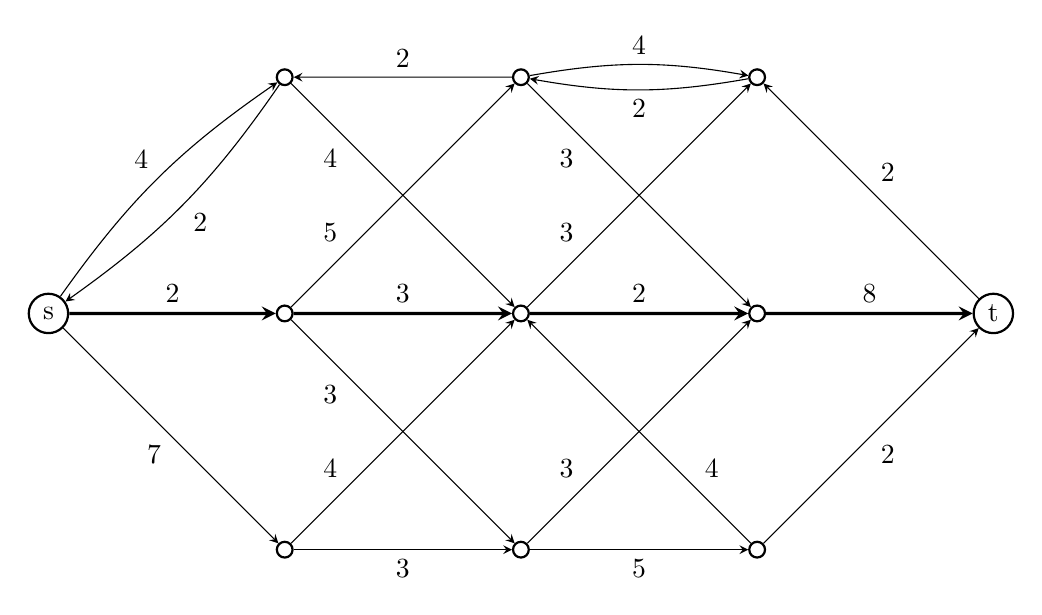
\begin{tikzpicture}[scale=1.5, >=stealth, bend angle=10]
    \node[st] (s) at (0,2) {s};
    \node[we] (a) at (2,0) {}; \node[we] (b) at (2,2) {}; \node[we] (c) at (2,4) {}; 
    \node[we] (d) at (4,0) {}; \node[we] (e) at (4,2) {}; \node[we] (f) at (4,4) {}; 
    \node[we] (g) at (6,0) {}; \node[we] (h) at (6,2) {}; \node[we] (i) at (6,4) {}; 
    \node[st] (t) at (8,2) {t};
    \draw[->] (s) to[edge label'=7, pos=.50] (a);
    \draw[->, very thick] (s) to[edge label =2, pos=.50] (b);
    \draw[->] (s) to[bend left, edge label =4, pos=.50] (c);
    \draw[<-] (s) to[bend right, edge label'=2, pos=.50] (c);
    \draw[->] (a) to[edge label'=3, pos=.50] (d);
    \draw[->, very thick] (b) to[edge label =3, pos=.50] (e);
    \draw[<-] (c) to[edge label =2, pos=.50] (f);
    \draw[->] (a) to[edge label =4, pos=.25] (e);
    \draw[->] (b) to[edge label =5, pos=.25] (f);
    \draw[->] (c) to[edge label'=4, pos=.25] (e);
    \draw[->] (b) to[edge label'=3, pos=.25] (d);
    \draw[->] (d) to[edge label'=5, pos=.50] (g);
    \draw[->, very thick] (e) to[edge label =2, pos=.50] (h);
    \draw[->] (f) to[bend left, edge label =4, pos=.50] (i);
    \draw[<-] (f) to[bend right, edge label'=2, pos=.50] (i);
    \draw[->] (d) to[edge label =3, pos=.25] (h);
    \draw[->] (e) to[edge label =3, pos=.25] (i);
    \draw[->] (f) to[edge label'=3, pos=.25] (h);
    \draw[<-] (e) to[edge label =4, pos=.75] (g);
    \draw[->] (g) to[edge label'=2, pos=.50] (t);
    \draw[->, very thick] (h) to[edge label =8, pos=.50] (t);
    \draw[<-] (i) to[edge label =2, pos=.50] (t);    
  \end{tikzpicture}
  \newpage
  %%%%%%%%%%%%%% THIRD PASS %%%%%%%%%%%%%%
  \subsection*{Third Pass}
  
  Original Network:\\
	\hfill
 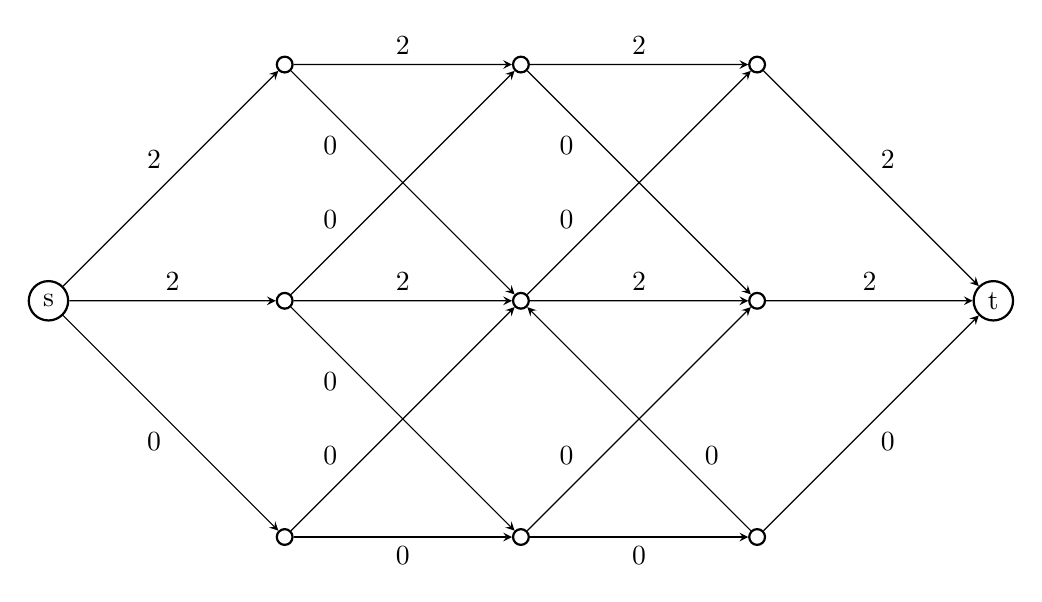
\begin{tikzpicture}[scale=1.5, >=stealth]
    \node[st] (s) at (0,2) {s};
    \node[we] (a) at (2,0) {}; \node[we] (b) at (2,2) {}; \node[we] (c) at (2,4) {}; 
    \node[we] (d) at (4,0) {}; \node[we] (e) at (4,2) {}; \node[we] (f) at (4,4) {}; 
    \node[we] (g) at (6,0) {}; \node[we] (h) at (6,2) {}; \node[we] (i) at (6,4) {}; 
    \node[st] (t) at (8,2) {t};
    \draw[->] (s) to[edge label'=0, pos=.50] (a);
    \draw[->] (s) to[edge label =2, pos=.50] (b);
    \draw[->] (s) to[edge label =2, pos=.50] (c);
    \draw[->] (a) to[edge label'=0, pos=.50] (d);
    \draw[->] (b) to[edge label =2, pos=.50] (e);
    \draw[->] (c) to[edge label =2, pos=.50] (f);
    \draw[->] (a) to[edge label =0, pos=.25] (e);
    \draw[->] (b) to[edge label =0, pos=.25] (f);
    \draw[->] (c) to[edge label'=0, pos=.25] (e);
    \draw[->] (b) to[edge label'=0, pos=.25] (d);
    \draw[->] (d) to[edge label'=0, pos=.50] (g);
    \draw[->] (e) to[edge label =2, pos=.50] (h);
    \draw[->] (f) to[edge label =2, pos=.50] (i);
    \draw[->] (d) to[edge label =0, pos=.25] (h);
    \draw[->] (e) to[edge label =0, pos=.25] (i);
    \draw[->] (f) to[edge label'=0, pos=.25] (h);
    \draw[<-] (e) to[edge label =0, pos=.75] (g);
    \draw[->] (g) to[edge label'=0, pos=.50] (t);
    \draw[->] (h) to[edge label =2, pos=.50] (t);
    \draw[->] (i) to[edge label =2, pos=.50] (t);    
  \end{tikzpicture}
     \hspace*{\fill} 
    
  Residual Network:\\
    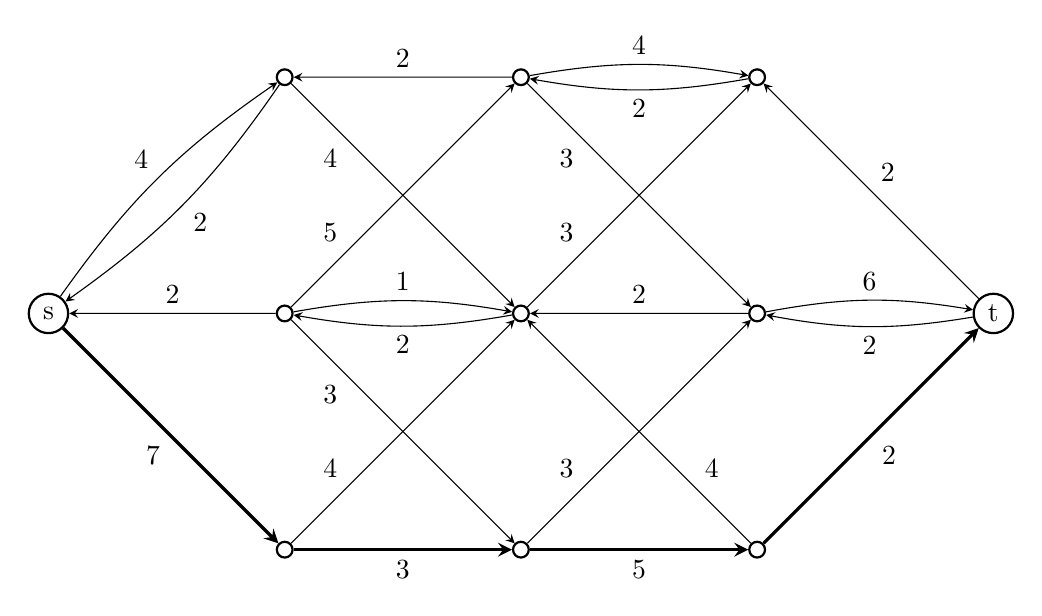
\begin{tikzpicture}[scale=1.5, >=stealth, bend angle=10]
    \node[st] (s) at (0,2) {s};
    \node[we] (a) at (2,0) {}; \node[we] (b) at (2,2) {}; \node[we] (c) at (2,4) {}; 
    \node[we] (d) at (4,0) {}; \node[we] (e) at (4,2) {}; \node[we] (f) at (4,4) {}; 
    \node[we] (g) at (6,0) {}; \node[we] (h) at (6,2) {}; \node[we] (i) at (6,4) {}; 
    \node[st] (t) at (8,2) {t};
    \draw[->, very thick] (s) to[edge label'=7, pos=.50] (a);
    \draw[<-] (s) to[edge label =2, pos=.50] (b);
    \draw[->] (s) to[bend left, edge label =4, pos=.50] (c);
    \draw[<-] (s) to[bend right, edge label'=2, pos=.50] (c);
    \draw[->, very thick] (a) to[edge label'=3, pos=.50] (d);
    \draw[->] (b) to[bend left, edge label =1, pos=.50] (e);
    \draw[<-] (b) to[bend right, edge label'=2, pos=.50] (e);
    \draw[<-] (c) to[edge label =2, pos=.50] (f);
    \draw[->] (a) to[edge label =4, pos=.25] (e);
    \draw[->] (b) to[edge label =5, pos=.25] (f);
    \draw[->] (c) to[edge label'=4, pos=.25] (e);
    \draw[->] (b) to[edge label'=3, pos=.25] (d);
    \draw[->,very thick] (d) to[edge label'=5, pos=.50] (g);
    \draw[<-] (e) to[edge label =2, pos=.50] (h);
    \draw[->] (f) to[bend left, edge label =4, pos=.50] (i);
    \draw[<-] (f) to[bend right, edge label'=2, pos=.50] (i);
    \draw[->] (d) to[edge label =3, pos=.25] (h);
    \draw[->] (e) to[edge label =3, pos=.25] (i);
    \draw[->] (f) to[edge label'=3, pos=.25] (h);
    \draw[<-] (e) to[edge label =4, pos=.75] (g);
    \draw[->, very thick] (g) to[edge label'=2, pos=.50] (t);
    \draw[->] (h) to[bend left, edge label =6, pos=.50] (t);
    \draw[<-] (h) to[bend right, edge label'=2, pos=.50] (t);
    \draw[<-] (i) to[edge label =2, pos=.50] (t);   
  \end{tikzpicture}
  \newpage
  %%%%%%%%%%%%%% FOURTH PASS %%%%%%%%%%%%%%
	\subsection*{Fourth Pass}
	
	Original Network:\\
	\hfill
 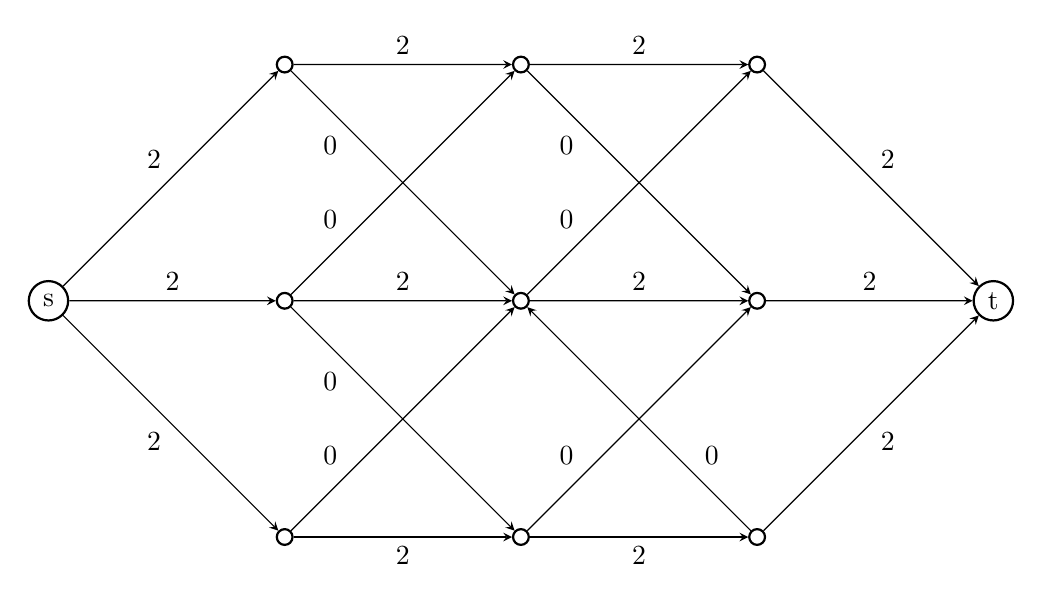
\begin{tikzpicture}[scale=1.5, >=stealth]
    \node[st] (s) at (0,2) {s};
    \node[we] (a) at (2,0) {}; \node[we] (b) at (2,2) {}; \node[we] (c) at (2,4) {}; 
    \node[we] (d) at (4,0) {}; \node[we] (e) at (4,2) {}; \node[we] (f) at (4,4) {}; 
    \node[we] (g) at (6,0) {}; \node[we] (h) at (6,2) {}; \node[we] (i) at (6,4) {}; 
    \node[st] (t) at (8,2) {t};
    \draw[->] (s) to[edge label'=2, pos=.50] (a);
    \draw[->] (s) to[edge label =2, pos=.50] (b);
    \draw[->] (s) to[edge label =2, pos=.50] (c);
    \draw[->] (a) to[edge label'=2, pos=.50] (d);
    \draw[->] (b) to[edge label =2, pos=.50] (e);
    \draw[->] (c) to[edge label =2, pos=.50] (f);
    \draw[->] (a) to[edge label =0, pos=.25] (e);
    \draw[->] (b) to[edge label =0, pos=.25] (f);
    \draw[->] (c) to[edge label'=0, pos=.25] (e);
    \draw[->] (b) to[edge label'=0, pos=.25] (d);
    \draw[->] (d) to[edge label'=2, pos=.50] (g);
    \draw[->] (e) to[edge label =2, pos=.50] (h);
    \draw[->] (f) to[edge label =2, pos=.50] (i);
    \draw[->] (d) to[edge label =0, pos=.25] (h);
    \draw[->] (e) to[edge label =0, pos=.25] (i);
    \draw[->] (f) to[edge label'=0, pos=.25] (h);
    \draw[<-] (e) to[edge label =0, pos=.75] (g);
    \draw[->] (g) to[edge label'=2, pos=.50] (t);
    \draw[->] (h) to[edge label =2, pos=.50] (t);
    \draw[->] (i) to[edge label =2, pos=.50] (t);    
  \end{tikzpicture}
   \hspace*{\fill} 
   
  Residual Network:\\
    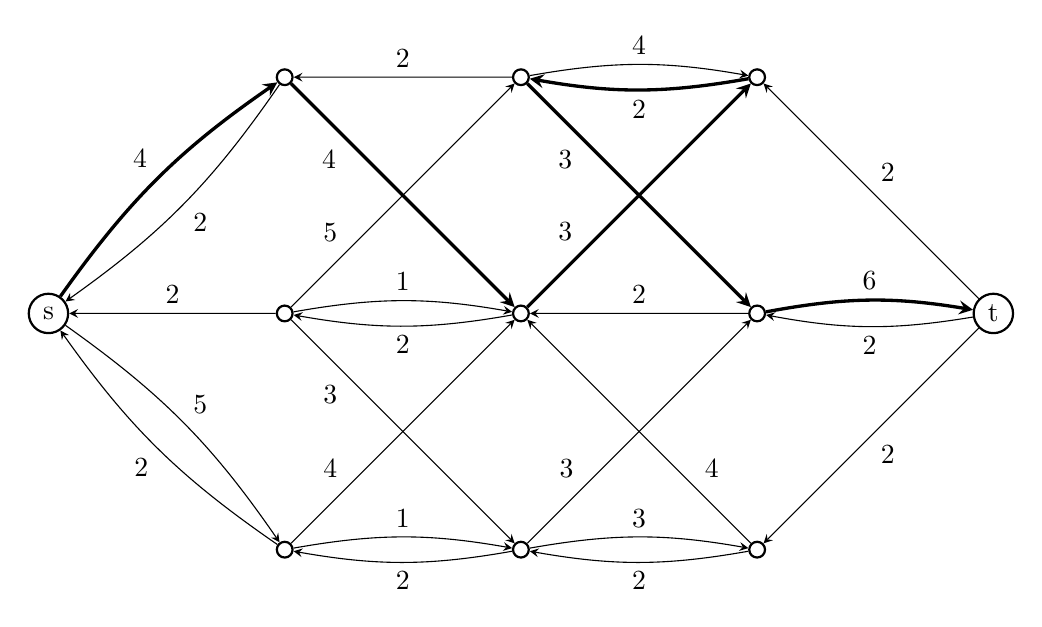
\begin{tikzpicture}[scale=1.5, >=stealth, bend angle=10]
    \node[st] (s) at (0,2) {s};
    \node[we] (a) at (2,0) {}; \node[we] (b) at (2,2) {}; \node[we] (c) at (2,4) {}; 
    \node[we] (d) at (4,0) {}; \node[we] (e) at (4,2) {}; \node[we] (f) at (4,4) {}; 
    \node[we] (g) at (6,0) {}; \node[we] (h) at (6,2) {}; \node[we] (i) at (6,4) {}; 
    \node[st] (t) at (8,2) {t};
    \draw[->] (s) to[bend left, edge label=5, pos=.50] (a);
    \draw[<-] (s) to[bend right, edge label'=2, pos=.50] (a);
    \draw[<-] (s) to[edge label =2, pos=.50] (b);
    \draw[->, very thick] (s) to[bend left, edge label =4, pos=.50] (c);
    \draw[<-] (s) to[bend right, edge label'=2, pos=.50] (c);
    \draw[->] (a) to[bend left, edge label=1, pos=.50] (d);
    \draw[<-] (a) to[bend right, edge label'=2, pos=.50] (d);
    \draw[->] (b) to[bend left, edge label =1, pos=.50] (e);
    \draw[<-] (b) to[bend right, edge label'=2, pos=.50] (e);
    \draw[<-] (c) to[edge label =2, pos=.50] (f);
    \draw[->] (a) to[edge label =4, pos=.25] (e);
    \draw[->] (b) to[edge label =5, pos=.25] (f);
    \draw[->, very thick] (c) to[edge label'=4, pos=.25] (e);
    \draw[->] (b) to[edge label'=3, pos=.25] (d);
    \draw[->] (d) to[bend left, edge label=3, pos=.50] (g);
    \draw[<-] (d) to[bend right, edge label'=2, pos=.50] (g);
    \draw[<-] (e) to[edge label =2, pos=.50] (h);
    \draw[->] (f) to[bend left, edge label =4, pos=.50] (i);
    \draw[<-, very thick] (f) to[bend right, edge label'=2, pos=.50] (i);
    \draw[->] (d) to[edge label =3, pos=.25] (h);
    \draw[->, very thick] (e) to[edge label =3, pos=.25] (i);
    \draw[->, very thick] (f) to[edge label'=3, pos=.25] (h);
    \draw[<-] (e) to[edge label =4, pos=.75] (g);
    \draw[<-] (g) to[edge label'=2, pos=.50] (t);
    \draw[->, very thick] (h) to[bend left, edge label =6, pos=.50] (t);
    \draw[<-] (h) to[bend right, edge label'=2, pos=.50] (t);
    \draw[<-] (i) to[edge label =2, pos=.50] (t);   
  \end{tikzpicture}
  \newpage
   %%%%%%%%%%%%%% FIFTH PASS %%%%%%%%%%%%%%
	\subsection*{Fifth Pass}
   Original Network:\\
	\hfill
 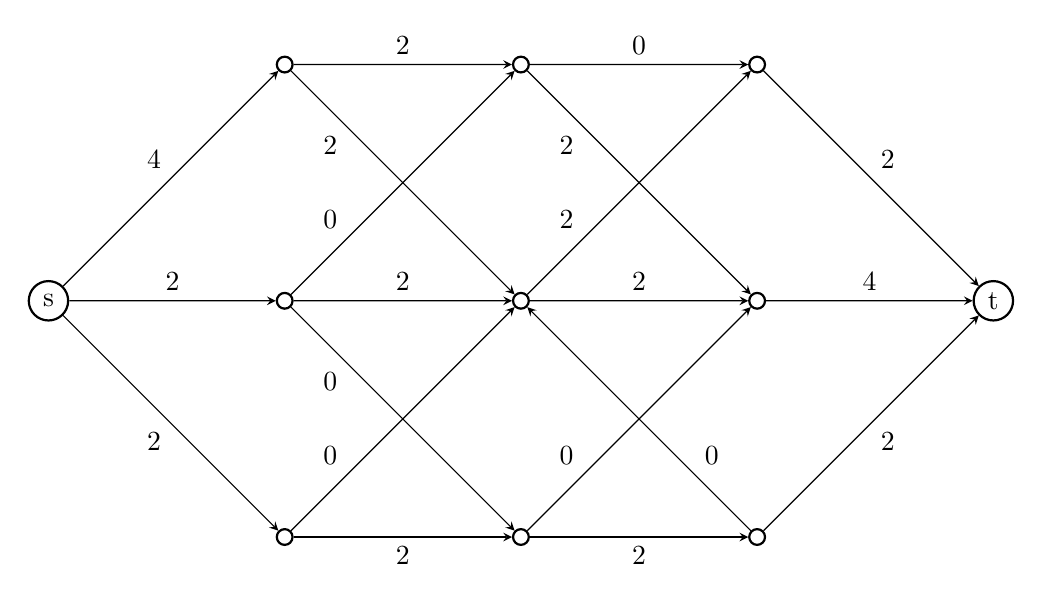
\begin{tikzpicture}[scale=1.5, >=stealth]
    \node[st] (s) at (0,2) {s};
    \node[we] (a) at (2,0) {}; \node[we] (b) at (2,2) {}; \node[we] (c) at (2,4) {}; 
    \node[we] (d) at (4,0) {}; \node[we] (e) at (4,2) {}; \node[we] (f) at (4,4) {}; 
    \node[we] (g) at (6,0) {}; \node[we] (h) at (6,2) {}; \node[we] (i) at (6,4) {}; 
    \node[st] (t) at (8,2) {t};
    \draw[->] (s) to[edge label'=2, pos=.50] (a);
    \draw[->] (s) to[edge label =2, pos=.50] (b);
    \draw[->] (s) to[edge label =4, pos=.50] (c);
    \draw[->] (a) to[edge label'=2, pos=.50] (d);
    \draw[->] (b) to[edge label =2, pos=.50] (e);
    \draw[->] (c) to[edge label =2, pos=.50] (f);
    \draw[->] (a) to[edge label =0, pos=.25] (e);
    \draw[->] (b) to[edge label =0, pos=.25] (f);
    \draw[->] (c) to[edge label'=2, pos=.25] (e);
    \draw[->] (b) to[edge label'=0, pos=.25] (d);
    \draw[->] (d) to[edge label'=2, pos=.50] (g);
    \draw[->] (e) to[edge label =2, pos=.50] (h);
    \draw[->] (f) to[edge label =0, pos=.50] (i);
    \draw[->] (d) to[edge label =0, pos=.25] (h);
    \draw[->] (e) to[edge label =2, pos=.25] (i);
    \draw[->] (f) to[edge label'=2, pos=.25] (h);
    \draw[<-] (e) to[edge label =0, pos=.75] (g);
    \draw[->] (g) to[edge label'=2, pos=.50] (t);
    \draw[->] (h) to[edge label =4, pos=.50] (t);
    \draw[->] (i) to[edge label =2, pos=.50] (t);    
  \end{tikzpicture}
   \hspace*{\fill} 
   
  Residual Network:\\
    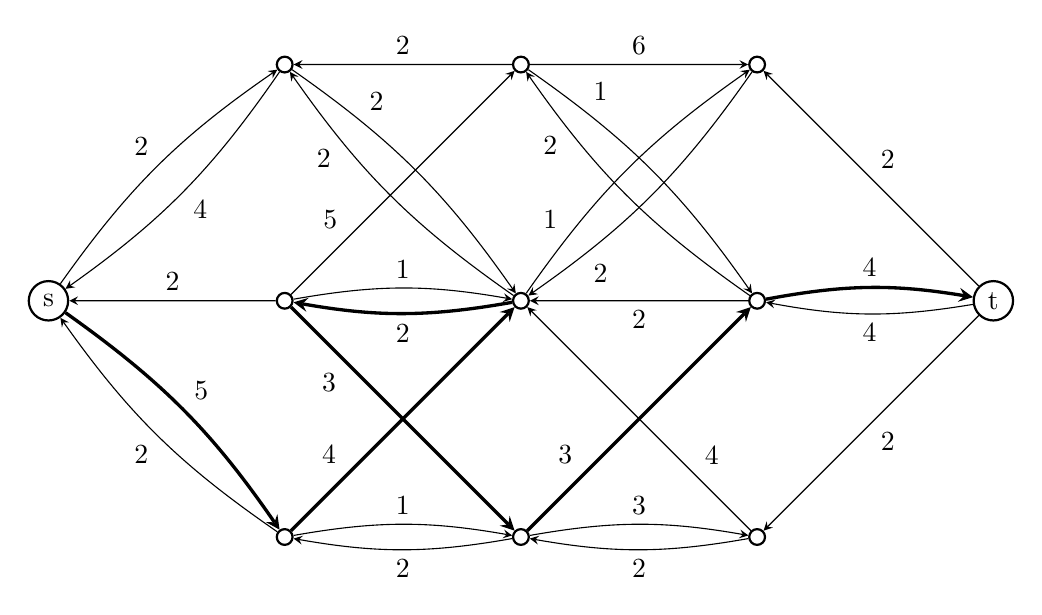
\begin{tikzpicture}[scale=1.5, >=stealth, bend angle=10]
    \node[st] (s) at (0,2) {s};
    \node[we] (a) at (2,0) {}; \node[we] (b) at (2,2) {}; \node[we] (c) at (2,4) {}; 
    \node[we] (d) at (4,0) {}; \node[we] (e) at (4,2) {}; \node[we] (f) at (4,4) {}; 
    \node[we] (g) at (6,0) {}; \node[we] (h) at (6,2) {}; \node[we] (i) at (6,4) {}; 
    \node[st] (t) at (8,2) {t};
    \draw[->, very thick] (s) to[bend left, edge label=5, pos=.50] (a);
    \draw[<-] (s) to[bend right, edge label'=2, pos=.50] (a);
    \draw[<-] (s) to[edge label =2, pos=.50] (b);
    \draw[->] (s) to[bend left, edge label =2, pos=.50] (c);
    \draw[<-] (s) to[bend right, edge label'=4, pos=.50] (c);
    \draw[->] (a) to[bend left, edge label=1, pos=.50] (d);
    \draw[<-] (a) to[bend right, edge label'=2, pos=.50] (d);
    \draw[->] (b) to[bend left, edge label =1, pos=.50] (e);
    \draw[<-, very thick] (b) to[bend right, edge label'=2, pos=.50] (e);
    \draw[<-] (c) to[edge label =2, pos=.50] (f);
    \draw[->, very thick] (a) to[edge label =4, pos=.25] (e);
    \draw[->] (b) to[edge label =5, pos=.25] (f);
    \draw[->] (c) to[bend left, edge label=2, pos=.25] (e);
    \draw[<-] (c) to[bend right, edge label'=2, pos=.25] (e);
    \draw[->, very thick] (b) to[edge label'=3, pos=.25] (d);
    \draw[->] (d) to[bend left, edge label=3, pos=.50] (g);
    \draw[<-] (d) to[bend right, edge label'=2, pos=.50] (g);
    \draw[<-] (e) to[edge label'=2, pos=.50] (h);
    \draw[->] (f) to[edge label =6, pos=.50] (i);
    %\draw[<-, very thick] (f) to[bend right, edge label'=2, pos=.50] (i);
    \draw[->, very thick] (d) to[edge label =3, pos=.25] (h);
    \draw[->] (e) to[bend left, edge label=1, pos=.20] (i);
    \draw[<-] (e) to[bend right, edge label'=2, pos=.20] (i);
    \draw[->] (f) to[bend left, edge label=1, pos=.20] (h);
    \draw[<-] (f) to[bend right, edge label'=2, pos=.20] (h);
    \draw[<-] (e) to[edge label =4, pos=.75] (g);
    \draw[<-] (g) to[edge label'=2, pos=.50] (t);
    \draw[->, very thick] (h) to[bend left, edge label =4, pos=.50] (t);
    \draw[<-] (h) to[bend right, edge label'=4, pos=.50] (t);
    \draw[<-] (i) to[edge label =2, pos=.50] (t);   
  \end{tikzpicture}
  \newpage
  %%%%%%%%%%%%%% SIXTH PASS %%%%%%%%%%%%%%
  \subsection*{Sixth Pass}
  Original Network:\\
	\hfill
 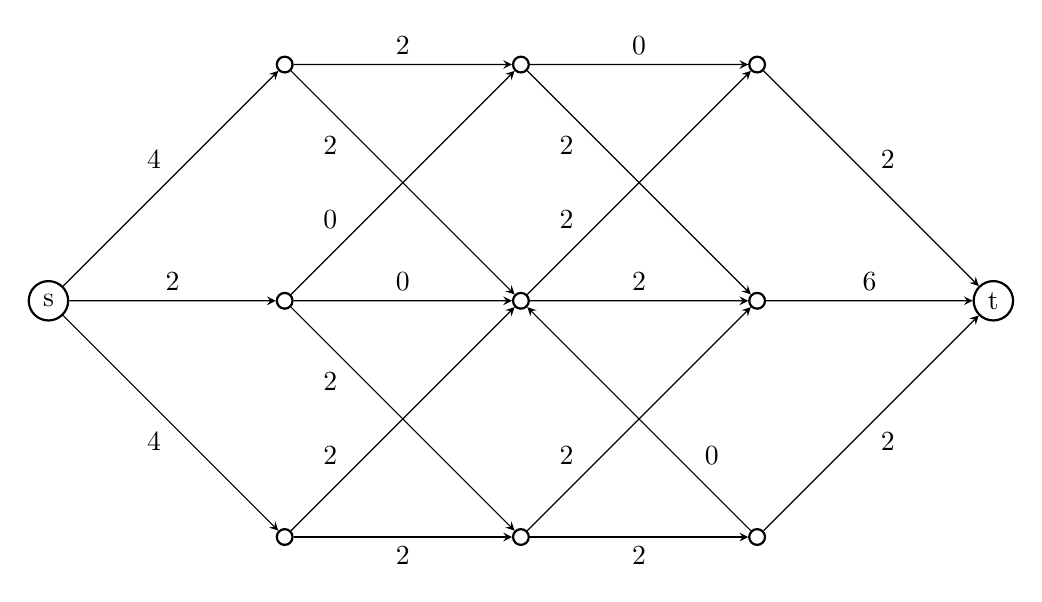
\begin{tikzpicture}[scale=1.5, >=stealth]
    \node[st] (s) at (0,2) {s};
    \node[we] (a) at (2,0) {}; \node[we] (b) at (2,2) {}; \node[we] (c) at (2,4) {}; 
    \node[we] (d) at (4,0) {}; \node[we] (e) at (4,2) {}; \node[we] (f) at (4,4) {}; 
    \node[we] (g) at (6,0) {}; \node[we] (h) at (6,2) {}; \node[we] (i) at (6,4) {}; 
    \node[st] (t) at (8,2) {t};
    \draw[->] (s) to[edge label'=4, pos=.50] (a);
    \draw[->] (s) to[edge label =2, pos=.50] (b);
    \draw[->] (s) to[edge label =4, pos=.50] (c);
    \draw[->] (a) to[edge label'=2, pos=.50] (d);
    \draw[->] (b) to[edge label =0, pos=.50] (e);
    \draw[->] (c) to[edge label =2, pos=.50] (f);
    \draw[->] (a) to[edge label =2, pos=.25] (e);
    \draw[->] (b) to[edge label =0, pos=.25] (f);
    \draw[->] (c) to[edge label'=2, pos=.25] (e);
    \draw[->] (b) to[edge label'=2, pos=.25] (d);
    \draw[->] (d) to[edge label'=2, pos=.50] (g);
    \draw[->] (e) to[edge label =2, pos=.50] (h);
    \draw[->] (f) to[edge label =0, pos=.50] (i);
    \draw[->] (d) to[edge label =2, pos=.25] (h);
    \draw[->] (e) to[edge label =2, pos=.25] (i);
    \draw[->] (f) to[edge label'=2, pos=.25] (h);
    \draw[<-] (e) to[edge label =0, pos=.75] (g);
    \draw[->] (g) to[edge label'=2, pos=.50] (t);
    \draw[->] (h) to[edge label =6, pos=.50] (t);
    \draw[->] (i) to[edge label =2, pos=.50] (t);    
  \end{tikzpicture}
   \hspace*{\fill} 
   
  Residual Network:\\
    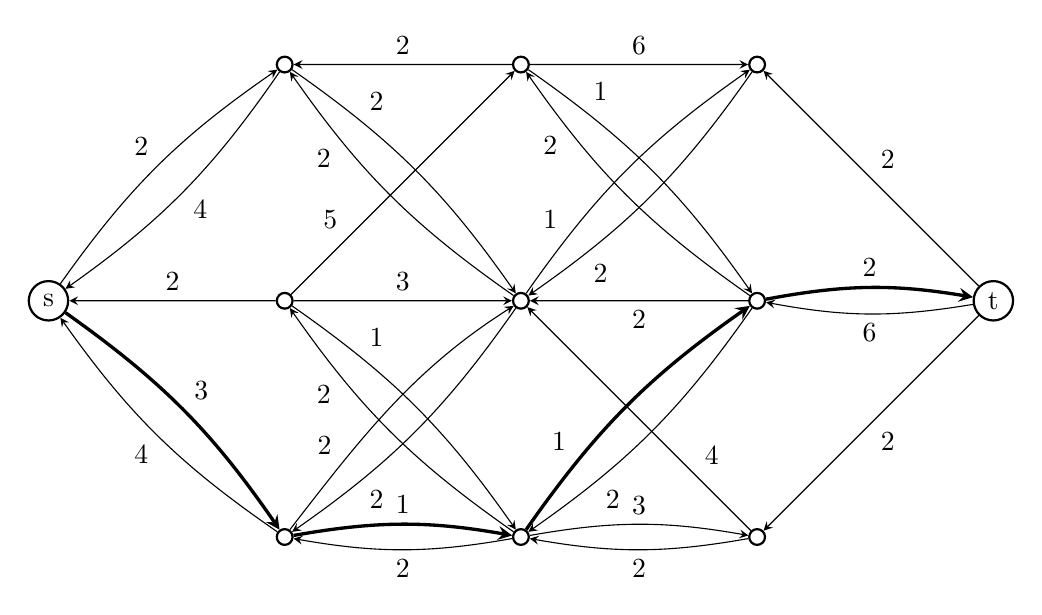
\begin{tikzpicture}[scale=1.5, >=stealth, bend angle=10]
    \node[st] (s) at (0,2) {s};
    \node[we] (a) at (2,0) {}; \node[we] (b) at (2,2) {}; \node[we] (c) at (2,4) {}; 
    \node[we] (d) at (4,0) {}; \node[we] (e) at (4,2) {}; \node[we] (f) at (4,4) {}; 
    \node[we] (g) at (6,0) {}; \node[we] (h) at (6,2) {}; \node[we] (i) at (6,4) {}; 
    \node[st] (t) at (8,2) {t};
    \draw[->, very thick] (s) to[bend left, edge label=3, pos=.50] (a);
    \draw[<-] (s) to[bend right, edge label'=4, pos=.50] (a);
    \draw[<-] (s) to[edge label =2, pos=.50] (b);
    \draw[->] (s) to[bend left, edge label =2, pos=.50] (c);
    \draw[<-] (s) to[bend right, edge label'=4, pos=.50] (c);
    \draw[->, very thick] (a) to[bend left, edge label=1, pos=.50] (d);
    \draw[<-] (a) to[bend right, edge label'=2, pos=.50] (d);
    \draw[->] (b) to[edge label =3, pos=.50] (e);
    %\draw[<-] (b) to[bend right, edge label'=2, pos=.50] (e);
    \draw[<-] (c) to[edge label =2, pos=.50] (f);
    \draw[->] (a) to[bend left, edge label=2, pos=.25] (e);
    \draw[<-] (a) to[bend right, edge label' =2, pos=.25] (e);
    \draw[->] (b) to[edge label =5, pos=.25] (f);
    \draw[->] (c) to[bend left, edge label=2, pos=.25] (e);
    \draw[<-] (c) to[bend right, edge label'=2, pos=.25] (e);
    \draw[->] (b) to[bend left, edge label=1, pos=.25] (d);
    \draw[<-] (b) to[bend right, edge label'=2, pos=.25] (d);
    \draw[->] (d) to[bend left, edge label=3, pos=.50] (g);
    \draw[<-] (d) to[bend right, edge label'=2, pos=.50] (g);
    \draw[<-] (e) to[edge label'=2, pos=.50] (h);
    \draw[->] (f) to[edge label =6, pos=.50] (i);
    %\draw[<-, very thick] (f) to[bend right, edge label'=2, pos=.50] (i);
    \draw[->, very thick] (d) to[bend left, edge label=1, pos=.25] (h);
    \draw[<-] (d) to[bend right, edge label'=2, pos=.25] (h);
    \draw[->] (e) to[bend left, edge label=1, pos=.20] (i);
    \draw[<-] (e) to[bend right, edge label'=2, pos=.20] (i);
    \draw[->] (f) to[bend left, edge label=1, pos=.20] (h);
    \draw[<-] (f) to[bend right, edge label'=2, pos=.20] (h);
    \draw[<-] (e) to[edge label =4, pos=.75] (g);
    \draw[<-] (g) to[edge label'=2, pos=.50] (t);
    \draw[->, very thick] (h) to[bend left, edge label =2, pos=.50] (t);
    \draw[<-] (h) to[bend right, edge label'=6, pos=.50] (t);
    \draw[<-] (i) to[edge label =2, pos=.50] (t);   
  \end{tikzpicture}
  \newpage
  %%%%%%%%%%%%%% SEVENTH PASS %%%%%%%%%%%%%%
  \subsection*{Seventh Pass}
  Original Network:\\
	\hfill
 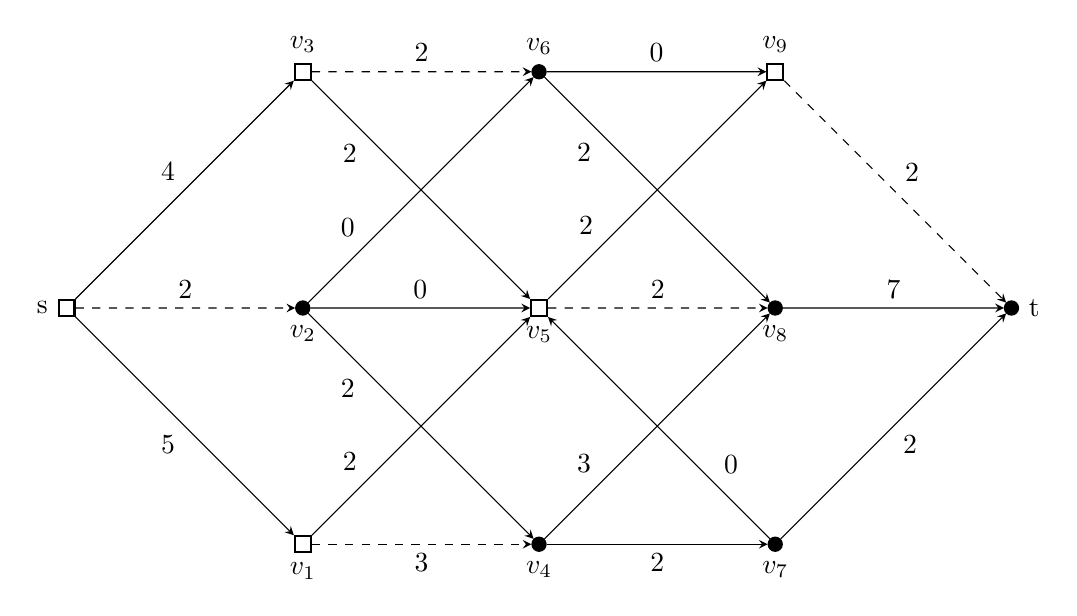
\begin{tikzpicture}[scale=1.5, >=stealth]
    \node[a, label=left:s] (s) at (0,2) {};
    \node[a, label=below:$v_1$] (a) at (2,0) {};
    \node[b, label=below:$v_2$] (b) at (2,2) {};
    \node[a, label=above:$v_3$] (c) at (2,4) {}; 
    \node[b, label=below:$v_4$] (d) at (4,0) {};
    \node[a, label=below:$v_5$] (e) at (4,2) {};
    \node[b, label=above:$v_6$] (f) at (4,4) {}; 
    \node[b, label=below:$v_7$] (g) at (6,0) {};
    \node[b, label=below:$v_8$] (h) at (6,2) {};
    \node[a, label=above:$v_9$] (i) at (6,4) {}; 
    \node[b, label=right:t] (t) at (8,2) {};
    \draw[->] (s) to[edge label'=5, pos=.50] (a);
    \draw[->, dashed] (s) to[edge label =2, pos=.50] (b);
    \draw[->] (s) to[edge label =4, pos=.50] (c);
    \draw[->, dashed] (a) to[edge label'=3, pos=.50] (d);
    \draw[->] (b) to[edge label =0, pos=.50] (e);
    \draw[->, dashed] (c) to[edge label =2, pos=.50] (f);
    \draw[->] (a) to[edge label =2, pos=.25] (e);
    \draw[->] (b) to[edge label =0, pos=.25] (f);
    \draw[->] (c) to[edge label'=2, pos=.25] (e);
    \draw[->] (b) to[edge label'=2, pos=.25] (d);
    \draw[->] (d) to[edge label'=2, pos=.50] (g);
    \draw[->, dashed] (e) to[edge label =2, pos=.50] (h);
    \draw[->] (f) to[edge label =0, pos=.50] (i);
    \draw[->] (d) to[edge label =3, pos=.25] (h);
    \draw[->] (e) to[edge label =2, pos=.25] (i);
    \draw[->] (f) to[edge label'=2, pos=.25] (h);
    \draw[<-] (e) to[edge label =0, pos=.75] (g);
    \draw[->] (g) to[edge label'=2, pos=.50] (t);
    \draw[->] (h) to[edge label =7, pos=.50] (t);
    \draw[->, dashed] (i) to[edge label =2, pos=.50] (t);    
  \end{tikzpicture}
   \hspace*{\fill} 
   
  Residual Network:\\
    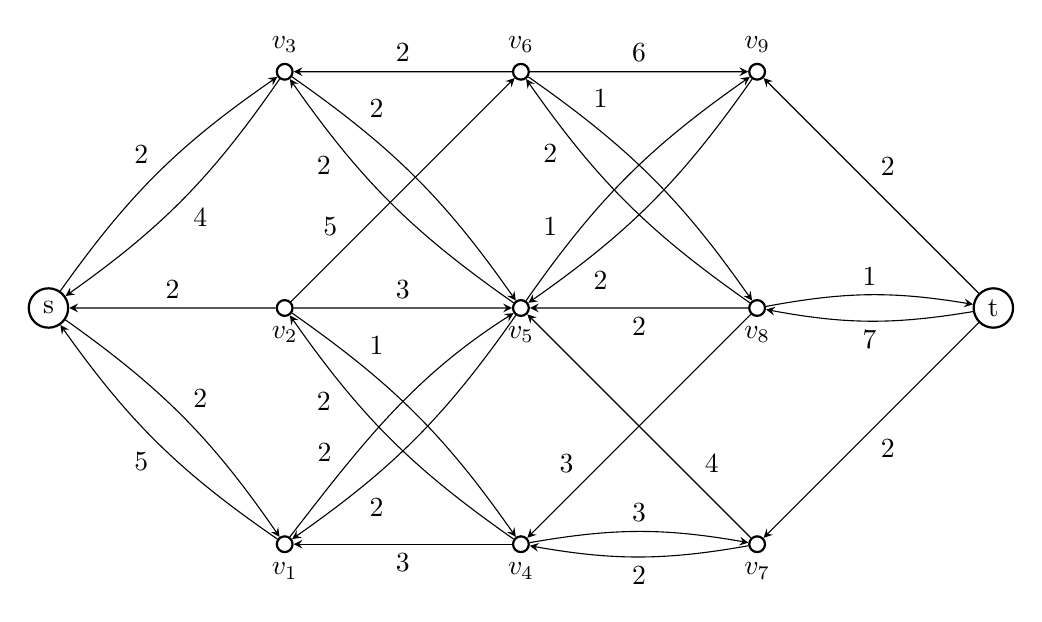
\begin{tikzpicture}[scale=1.5, >=stealth, bend angle=10]
    \node[st] (s) at (0,2) {s};
    \node[we, label=below:$v_1$] (a) at (2,0) {};
    \node[we, label=below:$v_2$] (b) at (2,2) {};
    \node[we, label=above:$v_3$] (c) at (2,4) {}; 
    \node[we, label=below:$v_4$] (d) at (4,0) {};
    \node[we, label=below:$v_5$] (e) at (4,2) {};
    \node[we, label=above:$v_6$] (f) at (4,4) {}; 
    \node[we, label=below:$v_7$] (g) at (6,0) {};
    \node[we, label=below:$v_8$] (h) at (6,2) {};
    \node[we, label=above:$v_9$] (i) at (6,4) {}; 
    \node[st] (t) at (8,2) {t};
    \draw[->] (s) to[bend left, edge label=2, pos=.50] (a);
    \draw[<-] (s) to[bend right, edge label'=5, pos=.50] (a);
    \draw[<-] (s) to[edge label =2, pos=.50] (b);
    \draw[->] (s) to[bend left, edge label =2, pos=.50] (c);
    \draw[<-] (s) to[bend right, edge label'=4, pos=.50] (c);
    %\draw[->, very thick] (a) to[bend left, edge label=1, pos=.50] (d);
    \draw[<-] (a) to[edge label'=3, pos=.50] (d);
    \draw[->] (b) to[edge label =3, pos=.50] (e);
    %\draw[<-] (b) to[bend right, edge label'=2, pos=.50] (e);
    \draw[<-] (c) to[edge label =2, pos=.50] (f);
    \draw[->] (a) to[bend left, edge label=2, pos=.25] (e);
    \draw[<-] (a) to[bend right, edge label' =2, pos=.25] (e);
    \draw[->] (b) to[edge label =5, pos=.25] (f);
    \draw[->] (c) to[bend left, edge label=2, pos=.25] (e);
    \draw[<-] (c) to[bend right, edge label'=2, pos=.25] (e);
    \draw[->] (b) to[bend left, edge label=1, pos=.25] (d);
    \draw[<-] (b) to[bend right, edge label'=2, pos=.25] (d);
    \draw[->] (d) to[bend left, edge label=3, pos=.50] (g);
    \draw[<-] (d) to[bend right, edge label'=2, pos=.50] (g);
    \draw[<-] (e) to[edge label'=2, pos=.50] (h);
    \draw[->] (f) to[edge label =6, pos=.50] (i);
    %\draw[<-, very thick] (f) to[bend right, edge label'=2, pos=.50] (i);
    %\draw[->, very thick] (d) to[bend left, edge label=1, pos=.25] (h);
    \draw[<-] (d) to[edge label=3, pos=.25] (h);
    \draw[->] (e) to[bend left, edge label=1, pos=.20] (i);
    \draw[<-] (e) to[bend right, edge label'=2, pos=.20] (i);
    \draw[->] (f) to[bend left, edge label=1, pos=.20] (h);
    \draw[<-] (f) to[bend right, edge label'=2, pos=.20] (h);
    \draw[<-] (e) to[edge label =4, pos=.75] (g);
    \draw[<-] (g) to[edge label'=2, pos=.50] (t);
    \draw[->] (h) to[bend left, edge label =1, pos=.50] (t);
    \draw[<-] (h) to[bend right, edge label'=7, pos=.50] (t);
    \draw[<-] (i) to[edge label =2, pos=.50] (t);   
  \end{tikzpicture}
  
\end{center}

\begin{enumerate}
\item The maximum flow has value 11. Formally 
\begin{equation*}
  |f| = f(\{s\}, \; V \backslash \{s\}) =  \sum_{\mathclap{\substack{(a,b) \; \; \in \\ <\{s\},\; V \backslash \{s\}>}}} f(a,b) - \sum_{\mathclap{\substack{(b,a) \; \; \in \\ <\{s\},\; V \backslash \{s\}>}}} f(b,a) = 2 + 2 + 7 = 11
\end{equation*}
\item A minimal cut  is indicated by the dashed lines on the original network. However, more formally, $<\{s, v_1, v_3, v_5, v_9 \}, \{t, v_2, v_4, v_6, v_7, v_8 \}>$ is the minimal cut, the edges being $(s, v_2), (v_1, v_4), (v_3, v_6), (v_9, t), (v_5, v_8)$. Finally the cut's capacity is 11, as 
\begin{equation*}
c(A,B) = \sum_{\mathclap{{(a,b) \; \; \in \; \; <A, B>}}} c(a,b) = 2+2+2+2+3 = 11
\end{equation*}
\end{enumerate}


\end{document}
